\model{Common Methods}

Classes are often used to represent abstract data types, such as \java{Color} or \java{Point}.
They are also used to represent objects in the real world, such as \java{CreditCard} (see \ref{credit-card.tex}) or \java{Person}.

\begin{center}
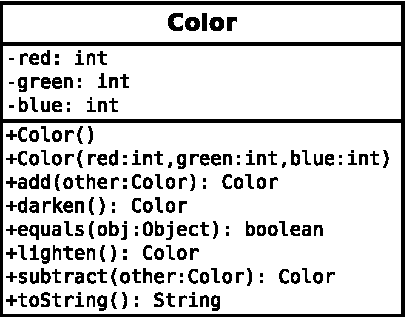
\includegraphics{Color.pdf}  % immutable
~~~~~
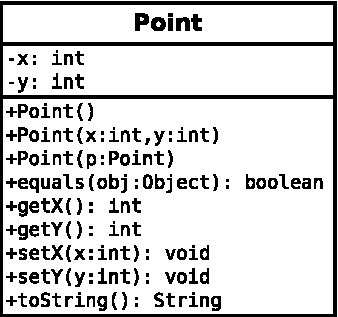
\includegraphics{Point.pdf}  % mutable
\end{center}

Classes generally include the following kinds of methods (in addition to others):
\begin{itemize}[itemsep=0pt]
\item \textbf{constructor} methods that initialize new objects
\item \textbf{accessor} methods (getters) that return attributes
\item \textbf{mutator} methods (setters) that modify attributes
\item \textbf{object} methods such as \java{equals} and \java{toString}
%\item \textbf{utility} methods which are generally static
\end{itemize}


\quest{20 min}


\Q Identify the constructors for the \java{Color} class.
What is the difference between them?
What arguments do they take?

\begin{answer}
There are two constructors: one that takes three integers for the RGB values, and other that takes a Color object. The latter is called a \emph{copy constructor}. Constructors do not return values.
\end{answer}


\Q What kind of constructor does the \java{Point} class have that the \java{Color} class does not?
What is the purpose of such a constructor?

\begin{answer}
The \java{Point} class also has a default constructor, which initializes attributes to their default value (most likely zero).
\end{answer}


\Q Identify an accessor method in the \java{Point} class.

\begin{enumerate}[itemsep=1pt]
\item Which instance variable does it get? \ans{{\tt this.x} or {\tt this.y}}
\item What arguments does the method take? \ans{none}
\item What does the method return? \ans{The value of \java{x} or \java{y}}
\end{enumerate}


\Q Identify a mutator method in the \java{Point} class.

\begin{enumerate}[itemsep=1pt]
\item Which instance variable does it set? \ans{{\tt this.x} or {\tt this.y}}
\item What arguments does the method take? \ans{The value of \java{x} or \java{y}}
\item What does the method return? \ans{nothing}
\end{enumerate}


\Q The \java{Color} class does not have accessors or mutators, but it provides methods that return lighter or darker \texttt{Color} objects.
Why do you think the class was designed this way?

\begin{answer}
Other than the constructor, there are no methods that change the \texttt{red}, \texttt{green}, and \texttt{blue} values.
This design makes the class immutable, which means that objects can be reused.
The \java{String} class is also designed this way.
\end{answer}


\vspace{2em}
\textit{In the following questions, consider the implementation of the \java{equals} method from each class.}
\vspace{1ex}

\begin{minipage}[t]{0.53\linewidth}
\begin{tabular}{|l|}
\hline
\textbf{Point.java}
\end{tabular}
\begin{javalst}
public boolean equals(Object obj) {
    if (obj instanceof Color) {
        Color other = (Color) obj;
        return this.red == other.red
            && this.green == other.green
            && this.blue == other.blue;
    }
    return false;
}
\end{javalst}
\end{minipage}
\hfill
\begin{minipage}[t]{0.46\linewidth}
\begin{tabular}{|l|}
\hline
\textbf{Color.java}
\end{tabular}
\begin{javalst}
public boolean equals(Object obj) {
    if (obj instanceof Point) {
        Point p = (Point) obj;
        return this.x == p.x
            && this.y == p.y;
    }
    return false;
}
\end{javalst}
\end{minipage}


\Q TODO

\begin{answer}
TODO
\end{answer}


\Q TODO

\begin{answer}
TODO
\end{answer}
